% !TeX encoding = UTF-8

%% ------------------------------------------------------------------------
%% Copyright (C) 2021-2023 SJTUG
%% 
%% SJTUBeamer Example Document by SJTUG
%% 
%% SJTUBeamer Example Document is licensed under a
%% Creative Commons Attribution-NonCommercial-ShareAlike 4.0 International License.
%% 
%% You should have received a copy of the license along with this
%% work. If not, see <http://creativecommons.org/licenses/by-nc-sa/4.0/>.
%%
%% For a quick start, check out src/doc/sjtubeamerquickstart.tex
%% Join discussions: https://github.com/sjtug/SJTUBeamer/discussions
%% -----------------------------------------------------------------------

\documentclass[xcolor=table,dvipsnames,svgnames,aspectratio=169]{ctexbeamer}
% 可以通过 fontset=macnew / fontset=ubuntu / fontset=windows 选项切换字体集;
% 如遇无法显示的数学符号,尝试对 ctexbeamer 文档类添加 no-math 选项;
% 写纯英文幻灯片可以改用 beamer 文档类。

\usepackage{tikz}
\usepackage[normalem]{ulem}
\usetikzlibrary{arrows}
\usepackage{amsmath}
\usepackage{graphicx}
\usepackage{hologo}
\usepackage{colortbl}
\usepackage{shapepar}
\usepackage{hyperxmp}
\usepackage{booktabs}
\usepackage{listings}
\usepackage{tipa}
\usepackage{multicol}
\usepackage{datetime2}
\usepackage{fontawesome5}
\usepackage{hyperref}
\usepackage{float}

% 参考文献设置,使用 style=gb7714-2015 样式为标准顺序编码制,
% 使用 style=gb7714-2015ay 样式可以改为著者-出版年制。
\usepackage[backend=biber,style=gb7714-2015]{biblatex}
\addbibresource{ref.bib}

% 该行指定了图像的额外搜索路径
\graphicspath{{figures/}}

\hypersetup{
  pdfcopyright       = {Licensed under CC-BY-SA 4.0. Some rights reserved.},
  pdflicenseurl      = {http://creativecommons.org/licenses/by-sa/4.0/},
  unicode            = true,
  psdextra           = true,
  pdfdisplaydoctitle = true
}

\pdfstringdefDisableCommands{
  \let\\\relax
  \let\quad\relax
  \let\hspace\@gobble
}

\renewcommand{\TeX}{\hologo{TeX}}
\renewcommand{\LaTeX}{\hologo{LaTeX}}
\newcommand{\BibTeX}{\hologo{BibTeX}}
\newcommand{\XeTeX}{\hologo{XeTeX}}
\newcommand{\pdfTeX}{\hologo{pdfTeX}}
\newcommand{\LuaTeX}{\hologo{LuaTeX}}
\newcommand{\MiKTeX}{\hologo{MiKTeX}}
\newcommand{\MacTeX}{Mac\hologo{TeX}}
\newcommand{\beamer}{\textsc{beamer}}
\newcommand{\XeLaTeX}{\hologo{Xe}\kern-.13em\LaTeX{}}
\newcommand{\pdfLaTeX}{pdf\LaTeX{}}
\newcommand{\LuaLaTeX}{Lua\LaTeX{}}
\def\TeXLive{\TeX{} Live}
\let\TL=\TeXLive

\newcommand{\SJTUThesis}{\textsc{SJTUThesis}}
\newcommand{\SJTUThesisVersion}{2.0.3}
\newcommand{\SJTUThesisDate}{2023/9/25}
\newcommand{\SJTUBeamer}{\textsc{SJTUBeamer}}
\newcommand{\SJTUBeamerVersion}{3.0.0}
\newcommand{\SJTUBeamerDate}{2022/11/22}

\newcommand\link[1]{\href{#1}{\faLink}}
\newcommand\pkg[1]{\texttt{#1}}

\def\cmd#1{\texttt{\color{structure}\footnotesize $\backslash$#1}}
\def\env#1{\texttt{\color{structure}\footnotesize #1}}
\def\cmdxmp#1#2#3{\small{\texttt{\color{structure}$\backslash$#1}\{#2\}
\hspace{1em}\\ $\Rightarrow$\hspace{1em} {#3}\par\vskip1em}}

\usetheme[min,blue,light,miniframes]{sjtubeamer}
% 使用 maxplus/max/min 切换标题页样式
% 使用 red/blue 切换主色调
% 使用 light/dark 切换亮/暗色模式
% 使用外样式关键词以获得不同的边栏样式
%   miniframes infolines  sidebar
%   default    smoothbars split	 
%   shadow     tree       smoothtree
% 使用 topright/bottomright 切换徽标位置
% 使用逗号分隔列表以同时使用多种选项

% \setbeamertemplate{background}{}
% 对于 max 主题,如果需要关闭正文背景图,请取消注释上一行。

% \tikzexternalize[prefix=build/]
% 如果您需要缓存 tikz 图像,请取消注释上一行,并在编译选项中添加 -shell-escape。

% \setbeamertemplate{sections/subsections in toc}[circle] % 使用普通的圆形目录结构

\lstset{
  language=[LaTeX]TeX,           % 更改高亮语言
  texcsstyle=*\color{cprimary},  % 只在高亮 LaTeX 语言时必须
  tabsize=2,
  basicstyle=\ttfamily\small,%
  keywordstyle=\color{cprimary},%
  stringstyle=\color{csecondary},%
  commentstyle=\color{ctertiary!50!gray},%
  breaklines,%
}

\author{答辩人:时涵天 \newline\newline 导师:秦通\newline\newline}
\institute[Pu Yuan Future Scholar Plan]{溥渊未来学者计划}
\date{\the\year 年 \the\month 月}
\subject{溥渊未来学者计划立项答辩}
\keywords{无人机,无线充电,能源}
\title[UM-SJTU JI \quad\quad Shi Hantian] % 页脚显示标题
{\textbf{无人机无线充电的硬件设计和自主导航}} % 首页标题

\subtitle{立项答辩}

\begin{document}

% 使用节目录
\AtBeginSection[]{
  \begin{frame}
    %% 使用传统节目录,也可以将 subsectionstyle=... 换成 hideallsubsections 以隐藏所有小节信息
    \tableofcontents[currentsection,subsectionstyle=show/show/hide]
    %% 或者使用节页
    % \sectionpage
  \end{frame}
}

% 使用小节目录
\AtBeginSubsection[]{		       % 在每小节开始
  \begin{frame}
    %% 使用传统小节目录
    \tableofcontents[currentsection,subsectionstyle=show/shaded/hide]
    %% 或者使用小节页
    % \subsectionpage
  \end{frame}
}

\maketitle

\begin{frame}{目录}
  \tableofcontents[hideallsubsections]	% 隐藏所有小节信息
\end{frame}

% !TeX encoding = UTF-8
% !TeX root = ../main.tex

%% ------------------------------------------------------------------------
%% Copyright (C) 2021-2023 SJTUG
%% 
%% SJTUBeamer Example Document by SJTUG
%% 
%% SJTUBeamer Example Document is licensed under a
%% Creative Commons Attribution-NonCommercial-ShareAlike 4.0 International License.
%% 
%% You should have received a copy of the license along with this
%% work. If not, see <http://creativecommons.org/licenses/by-nc-sa/4.0/>.
%% -----------------------------------------------------------------------

\section{选题背景及意义}

\begin{frame}[fragile]
  \frametitle{无人机应用的广泛性与重要性}

  无人机(Unmanned Aerial Vehicles, UAVs)因其卓越的灵活性和成本效益,已经在众多领域得到了广泛应用,包括但不限于:

  \begin{itemize}
    \item \textbf{农业监测}
    \begin{itemize}
      \item 高效监测农作物生长情况
      \item 评估病虫害
      \item 优化农业资源配置
    \end{itemize}

    \item \textbf{物流配送}
    \begin{itemize}
      \item 快速配送
      \item 特殊环境下的物资运输
    \end{itemize}

    \item \textbf{灾害救援}
    \begin{itemize}
      \item 提供现场情况
      \item 支持救援工作
    \end{itemize}
  \end{itemize}
  
\end{frame}

\begin{frame}[fragile]
  \frametitle{无人机续航能力的限制}
  尽管无人机应用广泛,但其续航能力受到电池容量和能量密度的限制。这一问题显著限制了无人机执行长时间和复杂任务的能力,特别是在以下情况下:
  \begin{itemize}
    \item \textbf{长时间巡航任务:}如大面积农田监测和森林火灾预警。
    \item \textbf{远距离物流配送:}如偏远地区的药品和急需物资配送。
    \item \textbf{连续环境监测:}如河流和湖泊的长期水质监测。
  \end{itemize}
\end{frame}

\begin{frame}[fragile]
  \frametitle{项目的创新性与应用价值}
  本项目旨在设计并实现一套无人机自动无线充电系统,其创新性和实际应用价值体现在:
  \begin{itemize}
    \item \textbf{无人机平台开发:}适合执行各种任务的四旋翼无人机
    \item \textbf{长时间巡航任务:}如大面积农田监测和森林火灾预警。
    \item \textbf{远距离物流配送:}如偏远地区的药品和急需物资配送。
    \item \textbf{连续环境监测:}如河流和湖泊的长期水质监测。
  \end{itemize}
\end{frame}

\begin{frame}
  \frametitle{项目意义}
  
  \begin{block}{1. 提高无人机的续航能力}
      \begin{itemize}
          \item \textbf{自动充电}:通过无线充电技术,无人机可以在任务过程中自动进行充电,无需更换电池,从而大幅延长其工作时间。
          \item \textbf{减少停机时间}:自动充电减少了无人机因电池耗尽而必须停机更换电池的时间,提高了工作效率。
      \end{itemize}
  \end{block}
  
  \begin{block}{2. 增强任务执行的灵活性}
      \begin{itemize}
          \item \textbf{适应多种任务需求}:无线充电技术使无人机能够在各种任务场景中灵活充电,适应长时间和复杂任务需求。
          \item \textbf{提升应急响应能力}:在紧急任务中,无人机能迅速恢复电力,持续执行任务。
      \end{itemize}
  \end{block}
\end{frame}
  
\begin{frame}
  \begin{block}{3. 推动无人机技术的智能化发展}
      \begin{itemize}
          \item \textbf{自主导航与对接}:开发无人机自动对接和精确降落算法,提高无人机的自主性和智能化水平。
          \item \textbf{系统集成与优化}:通过硬件和软件的集成与优化,实现无人机的全自动充电系统,推动无人机技术的发展。
      \end{itemize}
  \end{block}
  
  \begin{block}{4. 提升行业应用的效率和效果}
      \begin{itemize}
          \item \textbf{农业监测}:长时间、持续的监测提高农作物管理的精确度和及时性。
          \item \textbf{物流配送}:无人机在远距离和高频次的物流任务中能够持续运作,提高物流效率。
          \item \textbf{环境监测}:提供更长时间和更广范围的环境数据采集,提升环境保护和治理的效果。
      \end{itemize}
  \end{block}
\end{frame}

\begin{frame}
  \begin{block}{5. 促进新技术和新应用的开发}
      \begin{itemize}
          \item \textbf{跨领域技术融合}:结合无线充电技术和无人机技术,推动新技术的发展和应用。
          \item \textbf{引领产业创新}:为其他行业提供技术参考和创新思路,如自动驾驶车辆、智能家居设备的无线充电应用。
      \end{itemize}
  \end{block}


  \begin{block}{6. 节约资源和环保}
      \begin{itemize}
          \item \textbf{减少电池更换频率}:通过无线充电减少对电池的更换需求,延长电池使用寿命,降低资源消耗。
          \item \textbf{降低环境污染}:减少废旧电池的处理和更换,降低对环境的污染。
      \end{itemize}
  \end{block}
  
\end{frame}
% !TeX encoding = UTF-8
% !TeX root = ../main.tex

%% ------------------------------------------------------------------------
%% Copyright (C) 2021-2023 SJTUG
%% 
%% SJTUBeamer Example Document by SJTUG
%% 
%% SJTUBeamer Example Document is licensed under a
%% Creative Commons Attribution-NonCommercial-ShareAlike 4.0 International License.
%% 
%% You should have received a copy of the license along with this
%% work. If not, see <http://creativecommons.org/licenses/by-nc-sa/4.0/>.
%% -----------------------------------------------------------------------

\section{关键技术与实现难点}

\begin{frame}
  \frametitle{1. 技术调研与需求分析}
  
  \begin{block}{调研与分析内容}
    \begin{itemize}
      \item \textbf{现有解决方案调研}:长时间、持续的监测提高农作物管理的精确度和及时性。
      \item \textbf{技术需求分析}:无人机在远距离和高频次的物流任务中能够持续运作,提高物流效率。
      \item \textbf{技术挑战识别}:识别和评估可能遇到的技术挑战,如能量传输效率、充电稳定性、环境适应性等。
  \end{itemize}
  \end{block}
  \end{frame}
  
  \begin{frame}
  \frametitle{2. 硬件设计}
  
  \begin{block}{无线充电板设计}
      \begin{itemize}
          \item 设计与无人机电池兼容的无线充电板,确保高效能量传输。
          \item 考虑电磁兼容性和安全性,避免对无人机其他电子设备的干扰。
      \end{itemize}
  \end{block}
  
  \begin{block}{对接机构设计}
      \begin{itemize}
          \item 设计机械对接结构,确保无人机能够稳定地降落在充电板上。
          \item 设计电气连接系统,确保充电过程的稳定性和安全性。
      \end{itemize}
  \end{block}
  
  \end{frame}
  
  \begin{frame}
  \frametitle{3. 算法开发}
  
  \begin{block}{自动导航与定位算法}
      \begin{itemize}
          \item 开发无人机的自动导航和定位算法,实现精准的飞行路径规划。
          \item 确保无人机能够在不同环境下准确定位,避免障碍物。
      \end{itemize}
  \end{block}
  
  \begin{block}{自动对接算法}
      \begin{itemize}
          \item 开发自动对接算法,包括障碍物识别、降落点识别和精确降落控制。
          \item 确保无人机能够安全、准确地降落在充电板上,实现自动充电。
      \end{itemize}
  \end{block}
  
  \end{frame}
  
  \begin{frame}
  \frametitle{4. 系统集成}
  
  \begin{block}{硬件与软件集成}
      \begin{itemize}
          \item 将无线充电板、对接机构、导航与对接算法集成到一个完整的系统中。
          \item 确保硬件和软件之间的协调工作,实现系统的整体功能。
      \end{itemize}
  \end{block}
  
  \begin{block}{初步测试与调试}
      \begin{itemize}
          \item 进行系统的初步测试和调试,发现并解决潜在的问题。
          \item 优化系统性能,确保各组件的稳定运行。
      \end{itemize}
  \end{block}
  
  \end{frame}
  
  \begin{frame}
  \frametitle{5. 实地测试}
  
  \begin{block}{受控环境测试}
      \begin{itemize}
          \item 在受控环境中对无人机的自动充电系统进行测试,验证其功能和性能。
          \item 收集测试数据,分析系统的工作状态和充电效果。
      \end{itemize}
  \end{block}
  
  \begin{block}{数据分析与优化}
      \begin{itemize}
          \item 根据测试数据进行分析,找出系统的不足和改进点。
          \item 进一步优化系统,提高充电效率和系统稳定性。
      \end{itemize}
  \end{block}
  
  \end{frame}

% !TeX encoding = UTF-8
% !TeX root = ../main.tex

%% ------------------------------------------------------------------------
%% Copyright (C) 2021-2023 SJTUG
%% 
%% SJTUBeamer Example Document by SJTUG
%% 
%% SJTUBeamer Example Document is licensed under a
%% Creative Commons Attribution-NonCommercial-ShareAlike 4.0 International License.
%% 
%% You should have received a copy of the license along with this
%% work. If not, see <http://creativecommons.org/licenses/by-nc-sa/4.0/>.
%% -----------------------------------------------------------------------

\section{实现方法}

\begin{frame}[fragile]{全系统设计}
  \begin{figure}[H]
    \centering
    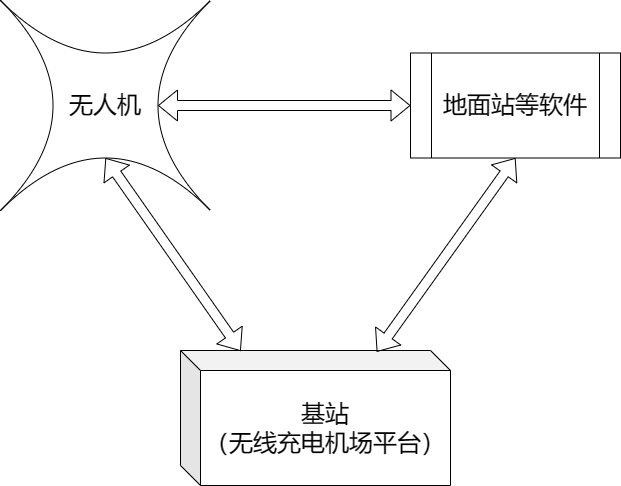
\includegraphics[height=0.7\textheight]{figures/full_system.png}
    \caption{全系统设计概念图}
  \end{figure}
\end{frame}

\begin{frame}[fragile]{基站系统设计}
  \begin{figure}[H]
    \centering
    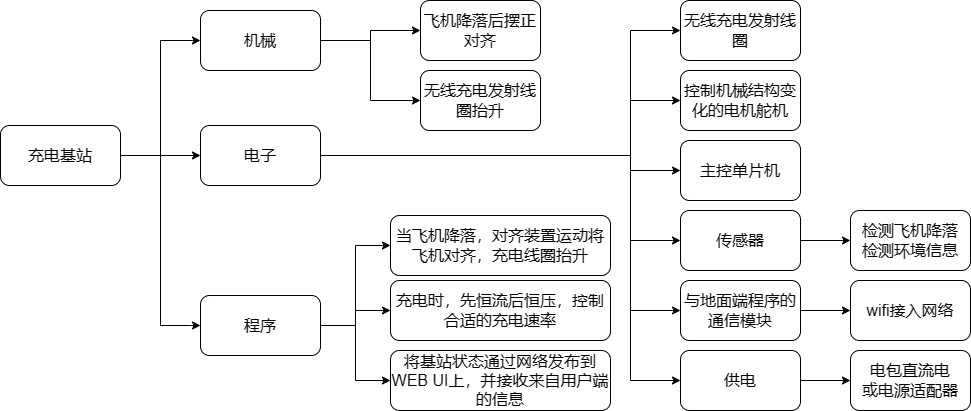
\includegraphics[height=0.7\textheight]{figures/base_station.png}
    \caption{基站系统设计示意图}
  \end{figure}
\end{frame}

\begin{frame}[fragile]{无人机通信系统设计}
  \begin{figure}[H]
    \centering
    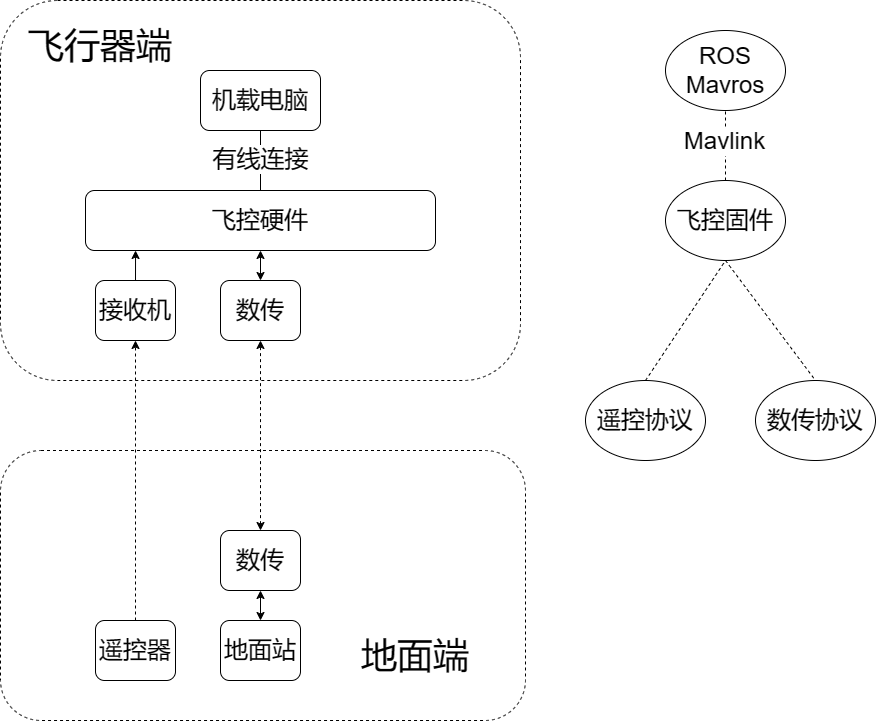
\includegraphics[height=0.7\textheight]{figures/communication_system.png}
    \caption{无人机通信系统设计示意图}
  \end{figure}
\end{frame}



% !TeX encoding = UTF-8
% !TeX root = ../main.tex

%% ------------------------------------------------------------------------
%% Copyright (C) 2021-2023 SJTUG
%% 
%% SJTUBeamer Example Document by SJTUG
%% 
%% SJTUBeamer Example Document is licensed under a
%% Creative Commons Attribution-NonCommercial-ShareAlike 4.0 International License.
%% 
%% You should have received a copy of the license along with this
%% work. If not, see <http://creativecommons.org/licenses/by-nc-sa/4.0/>.
%% -----------------------------------------------------------------------

\section{预期成果与应用}

\begin{frame}
  \begin{block}{推动无人机技术的智能化发展}
      \begin{itemize}
          \item \textbf{系统实现}:实现一套完整的无人机自动无线充电系统,包含无线充电平台基站、自动导航与对接算法。
          \item \textbf{集成与优化}:集成硬件、软件、算法,优化系统性能。
          \item \textbf{性能验证}:在实验室和实际环境中对系统进行全面测试,验证其充电效率、稳定性和可靠性。
      \end{itemize}
  \end{block}
  
  \begin{block}{技术成果整理与推广}
      \begin{itemize}
          \item \textbf{技术文档}:整理详细的技术文档,包括系统设计、实现过程、测试方法和结果分析等。
          \item \textbf{项目报告与总结}:编写项目报告,总结项目的实施过程、成果和经验。
          \item \textbf{学术论文与专利}:根据项目成果撰写学术论文或申请相关技术专利。
      \end{itemize}
  \end{block}
\end{frame}



\begin{frame}
  \frametitle{参考文献}
  \fontsize{8}{10}\selectfont
  \begin{itemize}
      \item T. Qin, P. Li and S. Shen, "VINS-Mono: A Robust and Versatile Monocular Visual-Inertial State Estimator," \textit{IEEE Transactions on Robotics}, vol. 34, no. 4, pp. 1004-1020, Aug. 2018. doi: 10.1109/TRO.2018.2853729.
      
      \item Y. Lin, F. Gao, T. Qin, et al., "Autonomous aerial navigation using monocular visual-inertial fusion," \textit{Journal of Field Robotics}, vol. 35, pp. 23–51, 2018. doi: 10.1002/rob.21732.
      
      \item T. Qin and S. Shen, "Online Temporal Calibration for Monocular Visual-Inertial Systems," \textit{2018 IEEE/RSJ International Conference on Intelligent Robots and Systems (IROS)}, Madrid, Spain, 2018, pp. 3662-3669. doi: 10.1109/IROS.2018.8593603.
      
      \item S. Obayashi, Y. Kanekiyo and T. Shijo, "UAV/Drone Fast Wireless Charging FRP Frustum Port for 85-kHz 50-V 10-A Inductive Power Transfer," \textit{2020 IEEE Wireless Power Transfer Conference (WPTC)}, Seoul, Korea (South), 2020, pp. 219-222. doi: 10.1109/WPTC48563.2020.9295562.
      
      \item M. C. Danciu, N. Yingta, I. Ur Rehman and S. Aleshaiker, "UAV Automated Charging Station and Charging Network in Smart Cities for Telemedicine Delivery," \textit{2023 IEEE International Smart Cities Conference (ISC2)}, Bucharest, Romania, 2023, pp. 1-6. doi: 10.1109/ISC257844.2023.10293330.
  \end{itemize}
  \end{frame}
  
  
\makebottom

\end{document}
